\documentclass[10pt]{exam}
\usepackage[phy]{template-for-exam}
\usepackage{tikz}
\usetikzlibrary{patterns}

\title{Marble Lab}
\author{Rohrbach}
\date{\today}

\begin{document}
\maketitle

\begin{questions}
  
  \question
    Set your black ramp on your lab station.  Pick one of the four tracks (use the same one each time.  Record which one you're using: \fillin[][10em]) and roll the marble down the track.  Use the photogate to determine how fast the marble is traveling when it gets to the bottom of the track.

    \begin{tabular}{|*5{c|}|c|}
      \hline
      Trial 1 (m/s)	&
      Trial 2 (m/s)	&
      Trial 3 (m/s)	&
      Trial 4 (m/s)	&
      Trial 5 (m/s)	&
      Average (m/s) \\
      \hline
      &&&&& \\[1.5em]
      \hline
  
    \end{tabular}

  
  \begin{EnvUplevel}
    Next you will be rolling the marble down and letting it hit the floor.  You will push the ramp to the end of the table.  {\bf Before you actually do this,} we are going to make the following calculations to predict how far from the table the marble will land.
  \end{EnvUplevel}
  	
  \question
    Below is a diagram showing the motion of the marble from the time it leaves the table until just before hitting the ground.  Label as many different variables as you can (such as displacement, time, velocity, etc.).
    
    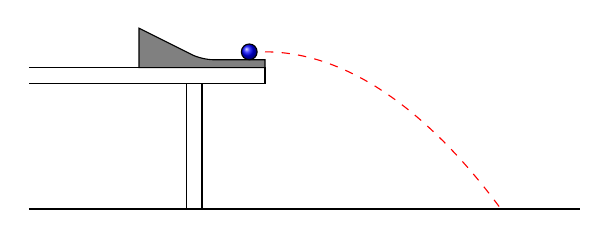
\begin{tikzpicture}
      \draw[thick] (0,0) -- (7,0);
      \draw (0,1.8)
        -- ++ (3,0)
        -- ++ (0,-.2)
        -- ++ (-3,0);
      \draw (2,0) rectangle (2.2,1.6);
      \draw[fill=gray] (3,1.9)
        -- ++(0,-.1)
        -- ++(-1.6,0) 
        -- ++(0,0.5)
        to[rounded corners] ++(.8,-.4)
        -- cycle;
      \draw[shading=ball] (2.8,2) circle (0.1);
      \draw[dashed,red] (3,2) parabola (6,0);

    \end{tikzpicture}
  
  \question
    Which direction is the marble travelling right when it leaves the table?  Would you call this the $x$-direction or the $y$-direction?
    \vspace{3em}
  
  \question
    What are our knowns (what do we already know, or can easily measure)?

    \begin{center}
      \begin{tabular}{c|c}
        $x$-direction & $y$-direction \\
        \hline \\
        \\[3em]
      \end{tabular}
    \end{center}
  
  \question
    For what values do we need to solve?
    \vspace{3em}
  
  \question
    How can we solve for the $x$-displacement of the marble?  Try it:

  \pagebreak
  
  \question
    We're going to see if you're right.  Push the ramp to the end of the table.  Place the weighing boat at the location you expect the marble to fall.  Measure carefully!!!
  
  \question
    Were you successful?  Explain sources of error in this experiment.  Also discuss what you could do in the future to minimize this error.
    \vs
  
  \uplevel{\section*{Conclusion}}
  
  \question
    What is the only variable that is the same in both the $x$- and the $y$- directions?  Why does it make sense that this variable is the same?
    \vs
  
  \question
    To find how far a projectile goes, you will usually solve this in two steps.  What are the two steps?
    \vs
\end{questions}





\end{document}